% ============================================================================
% Pedali.ma - Rapport Jalon 1 (Parties 1, 2 et 3)
% Compilation (depuis le dossier report/) :  pdflatex rapport.tex  (2 fois)
% Les images sont lues dans captures/ et les sorties brutes dans sorties/.
% ============================================================================
\documentclass[10pt,a4paper]{article}

\usepackage[T1]{fontenc}
\usepackage[utf8]{inputenc}
\usepackage[french]{babel}
\usepackage{lmodern}
\usepackage{microtype}
\usepackage[a4paper,margin=1.7cm,top=1.9cm,headheight=13pt]{geometry}
\usepackage{graphicx}
\usepackage{booktabs}
\usepackage{tabularx}
\usepackage{array}
\usepackage{float}
\usepackage[section]{placeins}
\usepackage[font=small,labelfont=bf]{caption}
\usepackage{subcaption}
\usepackage{xcolor}
\usepackage{listings}
\usepackage{fancyhdr}
\usepackage{enumitem}
\usepackage{tikz}
\usetikzlibrary{positioning,arrows.meta,fit}
\usepackage[hidelinks]{hyperref}

% ---------------------------------------------------------------- Binôme
\newcommand{\etudiantA}{Sara BASTA}
\newcommand{\etudiantB}{Siham CHAOUY}

% ---------------------------------------------------------------- Style
\definecolor{accent}{HTML}{1F4E79}
\definecolor{codebg}{HTML}{F5F7FA}
\definecolor{codeframe}{HTML}{C9D3DF}
\definecolor{kw}{HTML}{8A1F5B}
\definecolor{cm}{HTML}{5B7083}
\definecolor{st}{HTML}{2E7D32}

\graphicspath{{captures/}}
\setlist{itemsep=1pt,topsep=3pt}
\setlength{\parskip}{2pt}

\newcommand{\code}[1]{\texttt{\detokenize{#1}}}

\lstset{
  basicstyle=\ttfamily\scriptsize,
  backgroundcolor=\color{codebg},
  frame=single, rulecolor=\color{codeframe},
  breaklines=true, breakatwhitespace=false,
  postbreak=\mbox{\textcolor{cm}{$\hookrightarrow$}\space},
  columns=fullflexible, keepspaces=true,
  showstringspaces=false,
  xleftmargin=2pt, xrightmargin=2pt,
  aboveskip=4pt, belowskip=4pt,
  literate={é}{{\'e}}1 {è}{{\`e}}1 {ê}{{\^e}}1 {à}{{\`a}}1 {â}{{\^a}}1
           {ç}{{\c c}}1 {É}{{\'E}}1 {ô}{{\^o}}1 {î}{{\^i}}1 {û}{{\^u}}1
           {ù}{{\`u}}1 {×}{{$\times$}}1 {→}{{$\rightarrow$}}1
}
\lstdefinestyle{py}{language=Python,
  keywordstyle=\color{kw}\bfseries, commentstyle=\color{cm}\itshape,
  stringstyle=\color{st}}
\lstdefinestyle{sql}{language=SQL,
  keywordstyle=\color{kw}\bfseries, stringstyle=\color{st}}
\lstdefinestyle{out}{basicstyle=\ttfamily\scriptsize}

\pagestyle{fancy}
\fancyhf{}
\fancyhead[L]{\small\textcolor{accent}{Pedali.ma -- Jalon 1 (Parties 1 à 3)}}
\fancyhead[R]{\small EMSI -- Écosystème Big Data 2}
\fancyfoot[C]{\small\thepage}
\renewcommand{\headrulewidth}{0.4pt}

\hypersetup{pdftitle={Pedali.ma - Rapport Jalon 1},
            pdfauthor={Sara Basta, Siham Chaouy}}

% ============================================================================
\begin{document}

% ---------------------------------------------------------------- Page de garde
\begin{titlepage}
  \centering
  {\large EMSI -- École Marocaine des Sciences de l'Ingénieur\par}
  {\normalsize 5\textsuperscript{e} année -- Module \emph{Écosystème Big Data 2}\par}
  \vspace{3.2cm}
  {\color{accent}\rule{\linewidth}{1pt}\par}
  \vspace{0.5cm}
  {\Huge\bfseries Pedali.ma\par}
  \vspace{0.3cm}
  {\Large Plateforme Big Data pour un service de mobilité partagée\par}
  \vspace{0.4cm}
  {\large Suivi des trajets et analyse du réseau de stations\\
   avec Apache Spark, Kafka, GraphX et GraphFrames\par}
  \vspace{0.5cm}
  {\color{accent}\rule{\linewidth}{1pt}\par}
  \vspace{1.2cm}
  {\Large\bfseries Rapport -- Jalon 1\par}
  \vspace{0.2cm}
  {\large Partie 1 -- Mise en place du cluster et positionnement\\[1mm]
          Partie 2 -- Traitement batch avec SparkCore (RDD)\\[1mm]
          Partie 3 -- Spark SQL et DataFrames\par}
  \vfill
  {\large Réalisé en binôme par\par\vspace{0.2cm}
   {\Large \etudiantA \quad et \quad \etudiantB}\par}
  \vspace{1.2cm}
  {\normalsize Dépôt Git : \url{https://github.com/sara-basta/pedali-bigdata}\par}
  \vspace{0.3cm}
  {\normalsize Année universitaire 2026--2027 \quad·\quad Rendu du 22/11/2026\par}
\end{titlepage}


% ============================================================================
\section*{Introduction}
\addcontentsline{toc}{section}{Introduction}

Pedali.ma exploite des vélos, vélos électriques et trottinettes en libre-service à
Casablanca, Rabat, Marrakech et Tanger. Chaque changement d'état d'un trajet
(\code{RESERVED}, \code{UNLOCKED}, \code{ENDED}, \code{CANCELLED}, \code{FAULT_REPORTED})
produit un événement JSON. Le premier jalon met en place le cluster et analyse en
\emph{batch} un historique de trajets : d'abord avec l'API bas niveau (RDD), puis avec
l'API structurée (DataFrames et SQL). Le jalon 2 ajoutera le streaming Kafka, les couches
Silver/Gold en continu et l'analyse de graphes.

\paragraph{Jeu de données.} L'historique contient \textbf{51\,000 lignes} : 50\,000
événements, plus 1\,000 doublons (2\,\%, même \code{trip_id} et même \code{status}).
Environ 5\,\% des événements sont en retard (jusqu'à 15 minutes). Le référentiel compte
\textbf{400 stations}. Le \code{producer.py} de l'énoncé n'était pas dans notre dépôt au
moment des tests. Nous avons donc écrit \code{producer/gen_fake_history.py} et
\code{gen_fake_stations.py}. Ils respectent le schéma de l'énoncé : champs \code{null}
selon le statut, \code{battery_pct} nul pour les vélos classiques, retards et doublons. Ils
sont déterministes (graines fixes), ce qui rend tous les chiffres de ce rapport
reproductibles. Les tableaux viennent de l'exécution du 22/11/2026, conservée dans
\code{report/sorties/}. Les captures Spark UI datent des exécutions du 04/11 et du 09/11,
sur le même jeu de données.

\begin{figure}[!htbp]
\centering
\begin{tikzpicture}[
  node distance=5mm and 5mm,
  box/.style={draw=accent, rounded corners=2pt, fill=accent!6, align=center,
              font=\scriptsize, inner sep=3pt, minimum height=8mm},
  store/.style={box, fill=orange!8, draw=orange!70!black},
  fut/.style={box, dashed, fill=gray!5, draw=gray!70, text=gray!70!black},
  arr/.style={-{Stealth[length=2mm]}, thick, accent},
  farr/.style={-{Stealth[length=2mm]}, thick, dashed, gray!70}]
  \node[box] (gen) {Générateur\\\code{gen_fake_history.py}};
  \node[store, right=of gen] (bronze) {MinIO \code{lake/}\\\code{bronze/history/}};
  \node[box, right=of bronze, minimum width=3.4cm] (spark)
       {\textbf{Spark 3.5.3 standalone}\\Driver (\code{jupyter}) · Master\\2 Workers (2 cœurs, 2 Go)};
  \node[store, right=of spark] (silver) {MinIO \code{lake/}\\\code{silver/trips_history/}};
  \node[fut, below=of gen] (prod) {\code{producer.py}\\\code{--mode kafka}};
  \node[fut, right=of prod] (kafka) {Kafka (KRaft)\\topic \code{trips}, 3 partitions};
  \node[fut, below=of spark] (stream) {Structured Streaming\\GraphX / GraphFrames};
  \node[fut, right=of stream] (gold) {\code{silver/trips_clean/}\\\code{gold/} (Delta)};
  \draw[arr] (gen) -- node[above,font=\scriptsize]{upload} (bronze);
  \draw[arr] (bronze) -- node[above,font=\scriptsize]{S3A} (spark);
  \draw[arr] (spark) -- node[above,font=\scriptsize]{Parquet} (silver);
  \draw[farr] (prod) -- (kafka);
  \draw[farr] (kafka) -- (stream);
  \draw[farr] (stream) -- (gold);
\end{tikzpicture}
\caption{Chaîne mise en place. En trait plein, le chemin batch du jalon 1 ; en pointillés,
le chemin streaming et graphes du jalon 2 (Kafka et son topic sont déjà déployés).}
\label{fig:archi}
\end{figure}

% ============================================================================
\section{Partie 1 -- Mise en place du cluster et positionnement}

\subsection{Déploiement avec Docker Compose}

Toute la plateforme démarre avec \code{docker compose up -d --build}
(fichier \code{docker-compose.yml} du dépôt).

\begin{table}[!htbp]
\centering\small
\begin{tabularx}{\linewidth}{@{}l l X l@{}}
\toprule
\textbf{Service} & \textbf{Image} & \textbf{Rôle} & \textbf{Port(s)} \\
\midrule
\code{kafka} & \code{apache/kafka:3.8.0} & Broker et contrôleur en mode KRaft (sans ZooKeeper) & 9094 \\
\code{kafka-init} & \code{apache/kafka:3.8.0} & Crée le topic \code{trips} (3 partitions) puis s'arrête & -- \\
\code{minio} & \code{bitnamilegacy/minio} & Stockage objet S3 ; crée le bucket \code{lake} au démarrage & 9000 \\
\code{minio-console} & \code{bitnamilegacy/minio-object-browser} & Console web de MinIO & 9001 \\
\code{spark-master} & \code{pedali/spark:3.5.3-py3.11} & Cluster Manager \emph{standalone} & 8080, 7077 \\
\code{spark-worker-1/2} & \code{pedali/spark:3.5.3-py3.11} & Workers : 2 cœurs et 2 Go chacun & 8081, 8082 \\
\code{jupyter} & \code{pedali/spark:3.5.3-py3.11} & Driver : JupyterLab, scripts PySpark, Spark UI & 8888, 4040 \\
\bottomrule
\end{tabularx}
\caption{Services déployés.}
\end{table}

Quelques choix techniques :
\begin{itemize}
  \item \textbf{Une seule image} (\code{docker/spark/Dockerfile}) pour le Master, les Workers et le
    Driver : \code{python:3.11} + OpenJDK 17 + \code{pyspark==3.5.3}. PySpark refuse en effet
    de démarrer si le Python du Driver diffère de celui des Executors.
  \item \textbf{MinIO} n'est plus publié en image officielle. Nous utilisons l'image Bitnami
    archivée, avec la variable \code{MINIO_DEFAULT_BUCKETS=lake} qui crée le bucket au démarrage.
  \item \textbf{Accès S3A} : la fonction \code{get_spark()} de \code{notebooks/pedali_common.py}
    configure \code{hadoop-aws 3.3.4}, l'\emph{endpoint} \path{http://minio:9000} et le
    \emph{path-style access}. Toutes les parties lisent et écrivent donc \path{s3a://lake/...}.
\end{itemize}

\begin{lstlisting}[style=out,title={\footnotesize Vérification du topic Kafka (\texttt{kafka-topics.sh --describe --topic trips})}]
Topic: trips  TopicId: wvMF3XlSTva3ccs0K7Aftg  PartitionCount: 3  ReplicationFactor: 1
    Topic: trips  Partition: 0  Leader: 1  Replicas: 1  Isr: 1
    Topic: trips  Partition: 1  Leader: 1  Replicas: 1  Isr: 1
    Topic: trips  Partition: 2  Leader: 1  Replicas: 1  Isr: 1
\end{lstlisting}

\subsection{SparkSession connectée au Master}

Le script \code{notebooks/p1_cluster.py} crée la session sur \code{spark://spark-master:7077}.
Il attend ensuite que les deux executors soient enregistrés : juste après
\code{getOrCreate()}, \code{defaultParallelism} ne compterait que les cœurs déjà
disponibles. Il affiche alors les informations demandées (figure~\ref{fig:p1-session}).
\code{defaultParallelism = 4} correspond aux 2 Workers $\times$ 2 cœurs. Les deux
executors tournent sur les adresses des deux Workers (172.22.0.6 et 172.22.0.7).

\begin{figure}[!htbp]
\centering
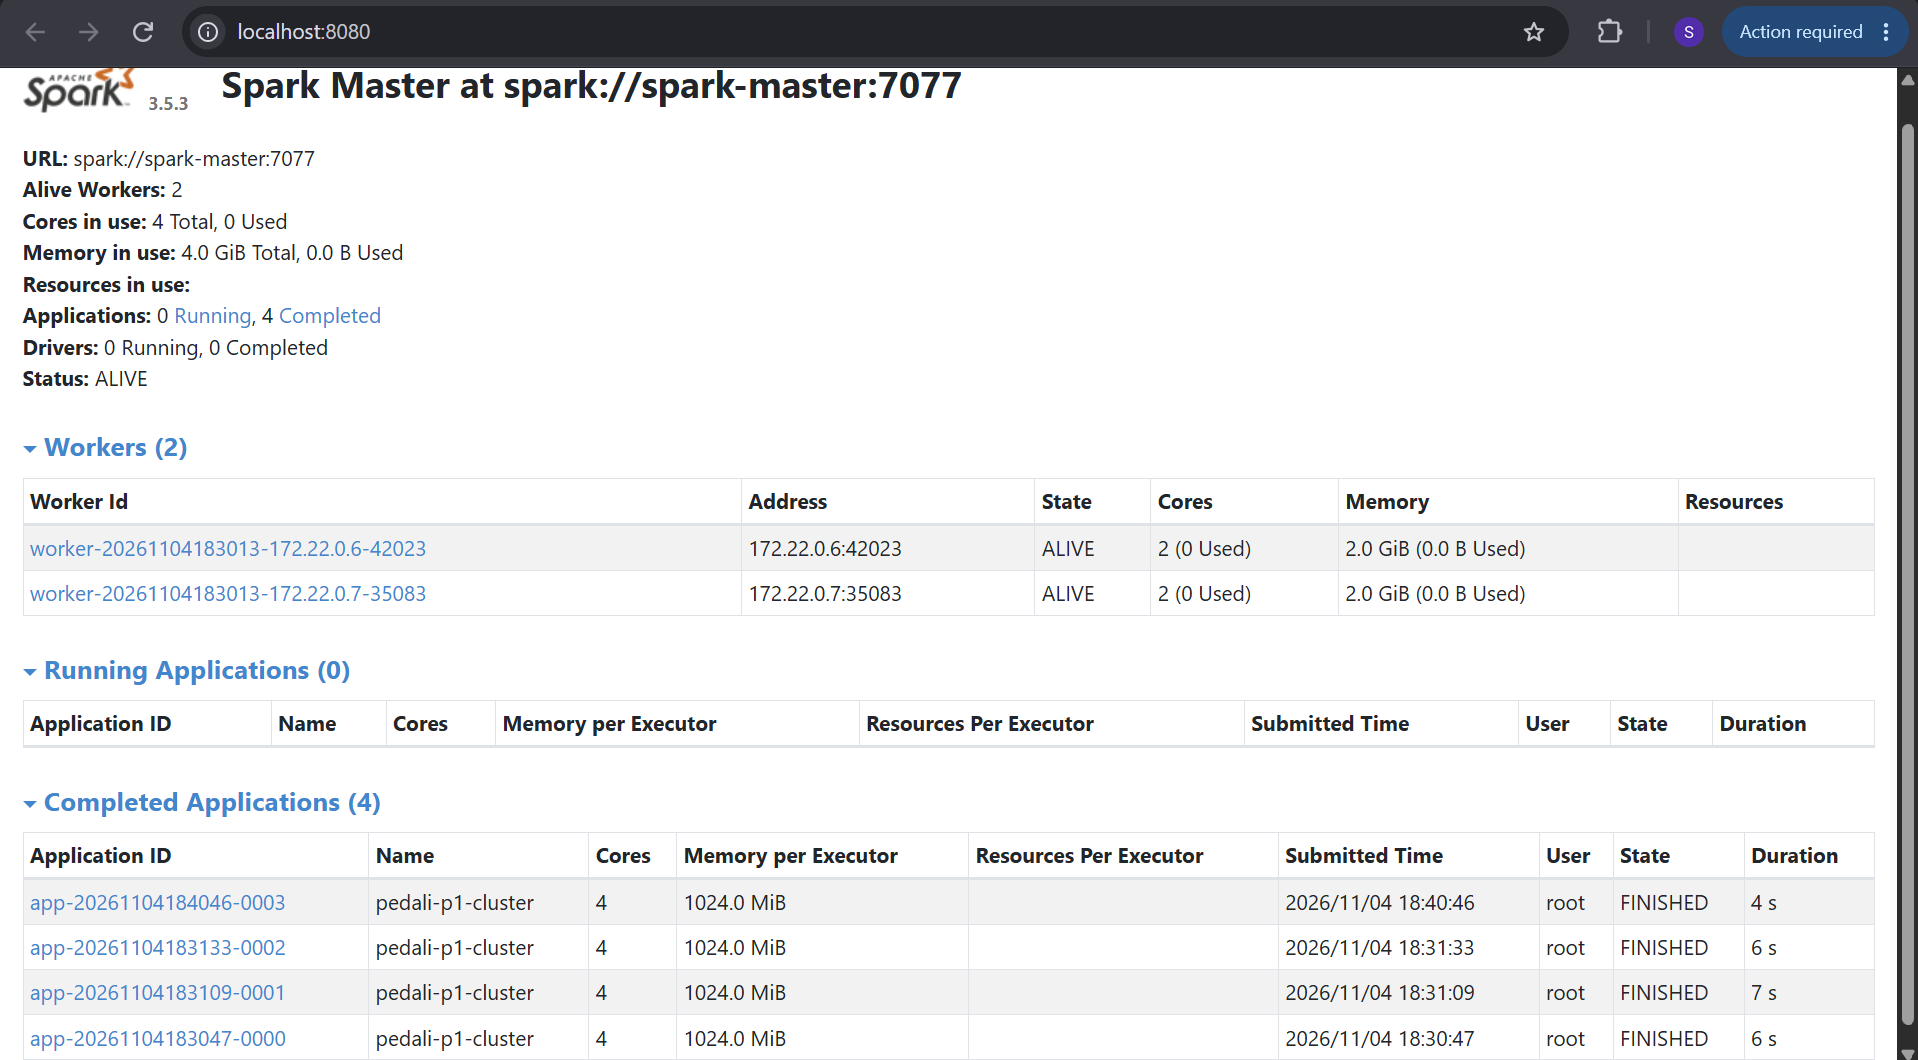
\includegraphics[width=0.62\linewidth]{p1_spark_master.png}
\caption{Interface Spark Master (port 8080) : 2 Workers \emph{ALIVE}, 4 cœurs et 4 Go au
total. Chaque application reçoit 4 cœurs et 1 Go par executor.}
\label{fig:p1-master}
\end{figure}

\begin{figure}[!htbp]
\centering
\begin{subfigure}[b]{0.47\linewidth}
  \centering
  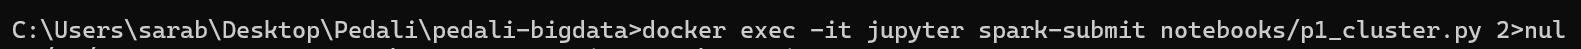
\includegraphics[width=\linewidth]{p1-sparksession-cmd.png}\\[2mm]
  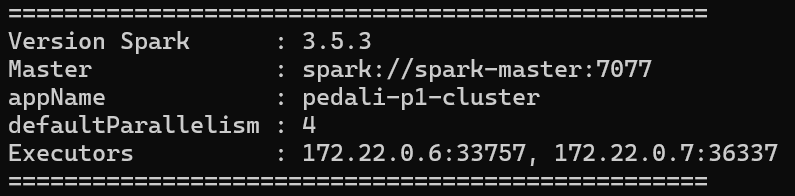
\includegraphics[width=\linewidth]{p1_sparksession-result.png}
  \caption{Lancement de \code{p1_cluster.py} et sortie.}
  \label{fig:p1-session}
\end{subfigure}\hfill
\begin{subfigure}[b]{0.5\linewidth}
  \centering
  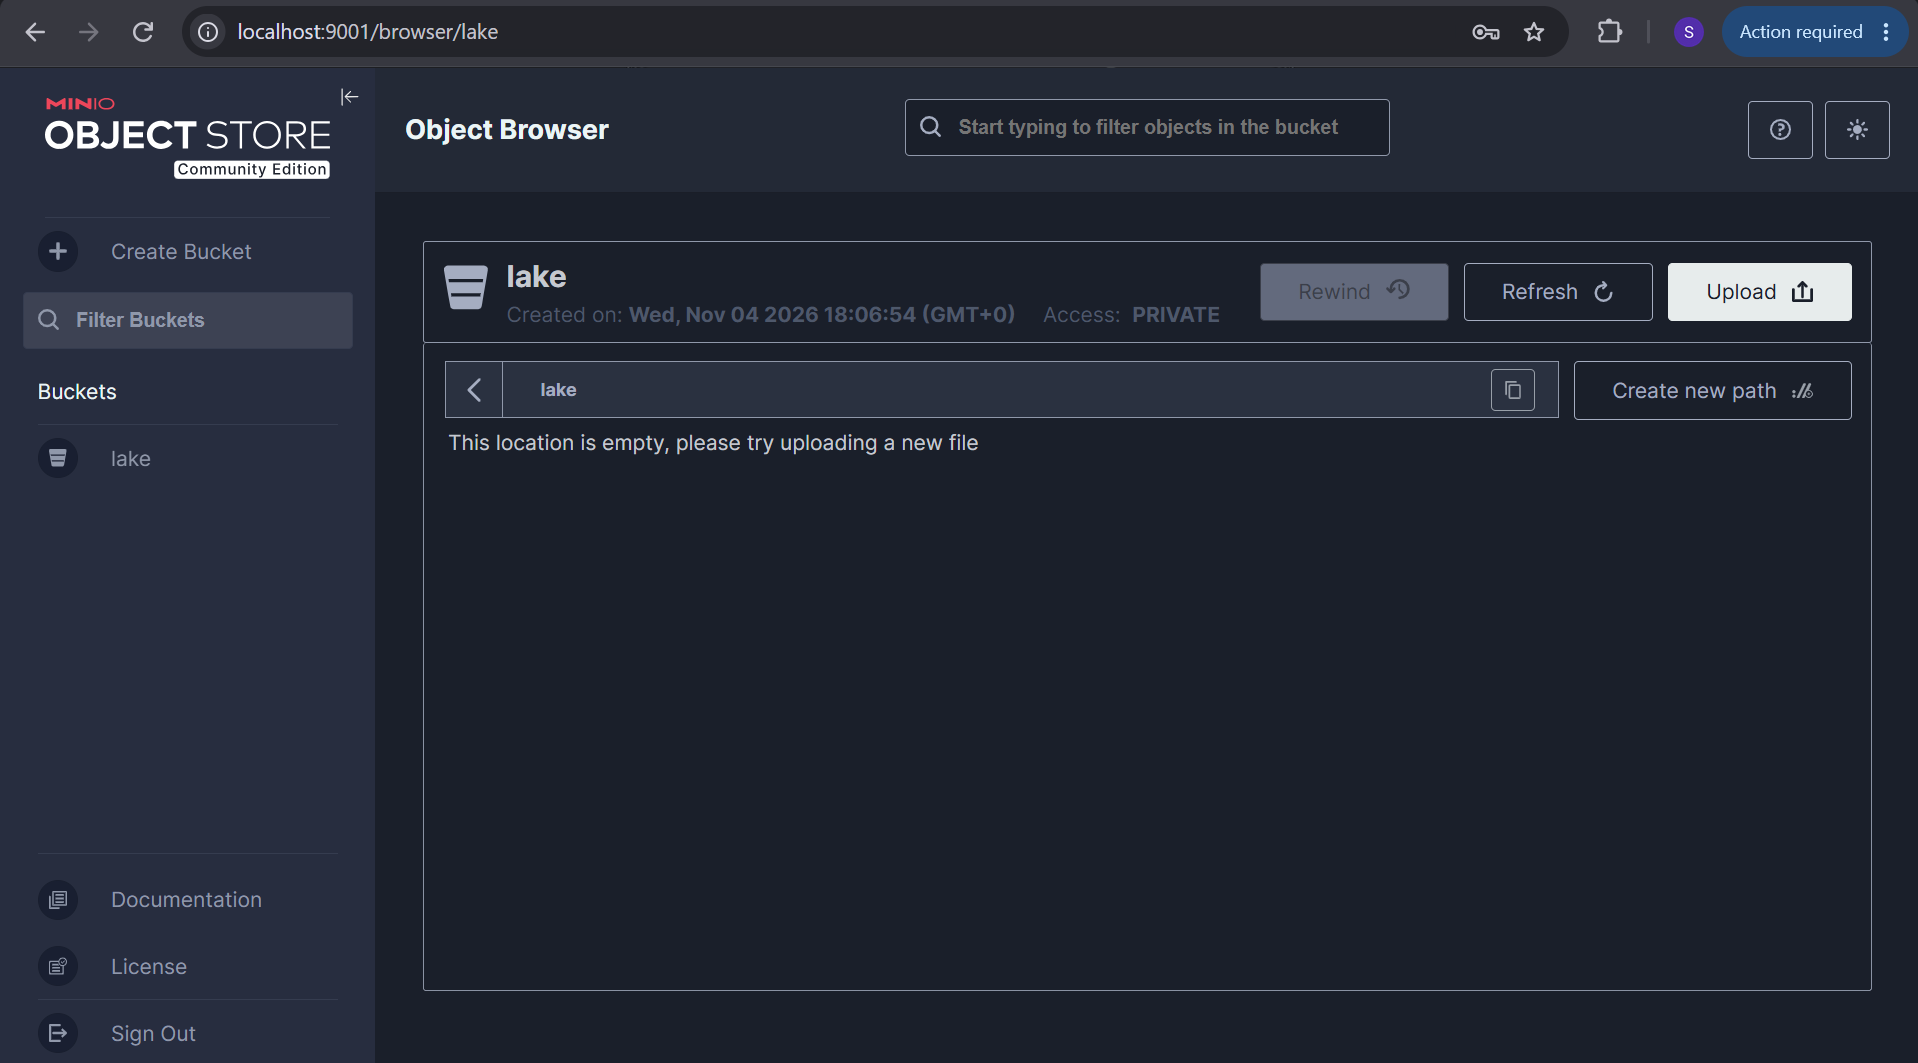
\includegraphics[width=\linewidth]{p1_minio_lake.png}
  \caption{Console MinIO (port 9001) : bucket \code{lake} créé.}
\end{subfigure}
\caption{Résultats attendus de la Partie 1.}
\end{figure}

\subsection{Rôle des composants dans notre déploiement}

\begin{itemize}
  \item \textbf{Driver} : c'est le processus Python lancé dans le conteneur \code{jupyter}
    (\code{spark.driver.host=jupyter}). Il exécute notre programme et transforme les
    opérations en un DAG de \emph{stages}. Il découpe ces stages en tâches (une par
    partition) et les envoie aux executors. Il récupère aussi les résultats des actions
    (\code{collect}, \code{count}) et expose la Spark UI sur le port 4040.
  \item \textbf{Cluster Manager} : le Master \emph{standalone} (\code{spark-master:7077}). Il
    connaît les ressources des Workers et, à la demande du Driver, demande à chaque Worker
    de lancer un executor (4 cœurs pour l'application). Il ne voit pas les données : il ne
    fait qu'allouer des ressources.
  \item \textbf{Workers et Executors} : chaque Worker (\code{spark-worker-1/2}) démarre un
    executor. C'est une JVM de 1 Go qui exécute les tâches sur 2 cœurs, avec des processus
    Python pour nos lambdas PySpark. Les executors lisent directement MinIO en S3A, gardent
    en mémoire les partitions mises en cache (RDD \code{ended} en Partie 2) et écrivent les
    fichiers de shuffle.
  \item \textbf{SparkContext} (porté par la \code{SparkSession}) : c'est le point d'entrée côté
    Driver. Il établit la connexion avec le Cluster Manager et crée les RDD
    (\code{sc.textFile}). Il porte la configuration (\code{appName}, packages S3A) et le
    \code{defaultParallelism}. Il n'en existe qu'un par application.
\end{itemize}

\subsection{Pourquoi Spark plutôt que MapReduce ?}

\begin{enumerate}
  \item \textbf{Résultats intermédiaires sur disque.} Avec Hadoop MapReduce, chaque job
    écrit sa sortie dans HDFS, répliquée 3 fois, et le job suivant la relit. Notre Partie 2
    enchaîne un filtrage, un dédoublonnage puis trois agrégations (CA, durée, top 5) sur les
    mêmes trajets : cela ferait quatre jobs MapReduce, chacun relisant le disque. Spark garde
    le DAG en mémoire. Avec \code{ended.cache()}, les trois agrégations réutilisent les
    données sans relire MinIO : la Spark UI marque l'étape de lecture comme
    \emph{skipped} et chaque agrégation prend environ une seconde
    (figure~\ref{fig:p2-ui}). C'est encore plus important pour les algorithmes itératifs de
    la Partie 6 (PageRank).
  \item \textbf{Traitement uniquement batch, à forte latence.} MapReduce ne traite que des
    lots déjà stockés, avec une latence de plusieurs minutes. Pedali a besoin d'indicateurs
    presque en temps réel à partir de Kafka (Parties 4 et 5). Spark Structured Streaming
    traite le flux en micro-batches de quelques secondes, avec la même API DataFrame que le
    batch. Plus largement, Spark couvre aussi les jointures avec le référentiel stations
    (Partie 3) et les analyses de graphes (Partie 6). Il regroupe tout
    cela dans un seul moteur et une seule API : Structured Streaming, Spark SQL, GraphX. Avec
    Hadoop, il faudrait assembler Storm, Hive et Giraph.
\end{enumerate}

% ============================================================================
\section{Partie 2 -- Traitement batch avec SparkCore (RDD)}

\subsection{Démarche}

Le script \code{notebooks/p2_rdd.py} enchaîne les étapes suivantes. Il lit
\path{s3a://lake/bronze/history/trips_history.jsonl} avec \code{sc.textFile()}. Il parse
chaque ligne avec \code{json.loads} dans un \code{flatMap} qui ignore les lignes invalides.
Il garde les trajets \code{ENDED} avec \code{filter}, puis supprime les doublons en gardant
un seul événement par \code{trip_id} (\code{reduceByKey}). Le RDD obtenu est mis en cache,
puis agrégé :

\begin{lstlisting}[style=py]
revenue = ended.map(lambda t: (t["city"], t["price_mad"] or 0.0)).reduceByKey(lambda a, b: a + b)
avg_duration = (ended.map(lambda t: ((t["city"], t["vehicle_type"]), t["duration_s"] or 0))
    .aggregateByKey((0, 0),                                   # (somme, nombre) en un seul passage
                    lambda acc, d: (acc[0] + d, acc[1] + 1),  # dans une partition
                    lambda a, b: (a[0] + b[0], a[1] + b[1]))  # entre partitions
    .mapValues(lambda s: s[0] / s[1]))
top5 = ended.map(lambda t: (t["start_station"], 1)).reduceByKey(lambda a, b: a + b) \
            .takeOrdered(5, key=lambda kv: -kv[1])
\end{lstlisting}

\subsection{Résultats}

Sur les 51\,000 lignes lues, il reste \textbf{14\,370 trajets terminés} distincts. Le
chiffre d'affaires total atteint \textbf{429\,563,25~MAD}, soit un panier moyen de
29,89~MAD.

\begin{table}[!htbp]
\centering\footnotesize
\begin{minipage}[t]{0.37\linewidth}\centering
\begin{tabular}{@{}lrrr@{}}
\toprule
\textbf{Ville} & \textbf{CA (MAD)} & \textbf{Part} & \textbf{Trajets} \\
\midrule
Casablanca & 192\,559,97 & 44,8\,\% & 6\,447 \\
Rabat      &  86\,641,49 & 20,2\,\% & 2\,918 \\
Marrakech  &  83\,975,32 & 19,5\,\% & 2\,813 \\
Tanger     &  66\,386,47 & 15,5\,\% & 2\,192 \\
\midrule
\textbf{Total} & \textbf{429\,563,25} & 100\,\% & 14\,370 \\
\bottomrule
\end{tabular}
\caption{Chiffre d'affaires par ville.}
\label{tab:ca}
\end{minipage}\hfill
\begin{minipage}[t]{0.36\linewidth}\centering
\begin{tabular}{@{}lrrr@{}}
\toprule
\textbf{Ville} & \textbf{BIKE} & \textbf{EBIKE} & \textbf{SCOOT.} \\
\midrule
Casablanca & 1\,154,2 & 1\,151,5 & 1\,143,9 \\
Marrakech  & 1\,101,7 & 1\,163,1 & 1\,135,1 \\
Rabat      & 1\,147,8 & 1\,142,3 & 1\,125,3 \\
Tanger     & 1\,190,1 & 1\,178,2 & 1\,142,6 \\
\bottomrule
\end{tabular}
\caption{Durée moyenne (secondes).}
\label{tab:duree}
\end{minipage}\hfill
\begin{minipage}[t]{0.22\linewidth}\centering
\begin{tabular}{@{}clr@{}}
\toprule
\textbf{\#} & \textbf{Station} & \textbf{Trajets} \\
\midrule
1 & S-CAS-001 & 269 \\
2 & S-CAS-003 & 250 \\
3 & S-CAS-002 & 238 \\
4 & S-CAS-004 & 232 \\
5 & S-CAS-005 & 232 \\
\bottomrule
\end{tabular}
\caption{Top 5 des départs.}
\label{tab:top5}
\end{minipage}
\end{table}

Casablanca représente 45\,\% des trajets et du CA, et le panier moyen est stable d'une ville
à l'autre (29,7 à 30,3~MAD). Les durées moyennes tournent autour de 19 minutes pour tous
les véhicules, ce qui est cohérent avec le générateur : il tire la durée dans une même loi
log-normale quel que soit le type de véhicule. Les cinq stations les plus utilisées sont à
Casablanca, la ville la plus active ; S-CAS-001 est la gare principale.

\subsection{Lineage, transformations et actions}

\begin{lstlisting}[style=out,title={\footnotesize \texttt{revenue.toDebugString()}}]
(2) PythonRDD[13] at collect at /opt/pedali/notebooks/p2_rdd.py:59 []
 |  MapPartitionsRDD[12] at mapPartitions at PythonRDD.scala:160 []
 |  ShuffledRDD[11] at partitionBy at NativeMethodAccessorImpl.java:0 []
 +-(2) PairwiseRDD[10] at reduceByKey at /opt/pedali/notebooks/p2_rdd.py:58 []
    |  PythonRDD[9] at reduceByKey at /opt/pedali/notebooks/p2_rdd.py:58 []
    |  PythonRDD[6] at RDD at PythonRDD.scala:53 []
    |      CachedPartitions: 2; MemorySize: 1068.5 KiB; DiskSize: 0.0 B
    |  MapPartitionsRDD[5] at mapPartitions at PythonRDD.scala:160 []
    |  ShuffledRDD[4] at partitionBy at NativeMethodAccessorImpl.java:0 []
    +-(2) PairwiseRDD[3] at reduceByKey at /opt/pedali/notebooks/p2_rdd.py:48 []
       |  PythonRDD[2] at reduceByKey at /opt/pedali/notebooks/p2_rdd.py:48 []
       |  s3a://lake/bronze/history/trips_history.jsonl MapPartitionsRDD[1] at textFile at ...
       |  s3a://lake/bronze/history/trips_history.jsonl HadoopRDD[0] at textFile at ...
\end{lstlisting}

Le lineage se lit de bas en haut. Chaque décrochage \code{+-} correspond à une dépendance
large (\code{ShuffledRDD}), donc à une frontière de stage. On y voit deux shuffles : le
dédoublonnage (ligne~48) et le CA par ville (ligne~58). Le RDD \code{ended} est en cache
(\code{CachedPartitions: 2}, environ 1~Mo). \code{(2)} est le nombre de partitions :
\code{textFile} en crée 2 par défaut pour un fichier de 16~Mo.
\begin{itemize}
  \item \textbf{Transformations (lazy)} : \code{textFile}, \code{flatMap}, \code{filter},
    \code{map}, \code{reduceByKey}, \code{aggregateByKey}, \code{mapValues}, \code{values},
    \code{cache}. Elles ne font que construire le graphe.
  \item \textbf{Actions} : \code{count}, \code{collect}, \code{takeOrdered}. Chacune déclenche
    un job, ce qui donne 5 jobs dans la Spark UI.
\end{itemize}

\subsection{DAG, stages et shuffle}

\begin{figure}[!htbp]
\centering
\begin{subfigure}[b]{\linewidth}\centering
  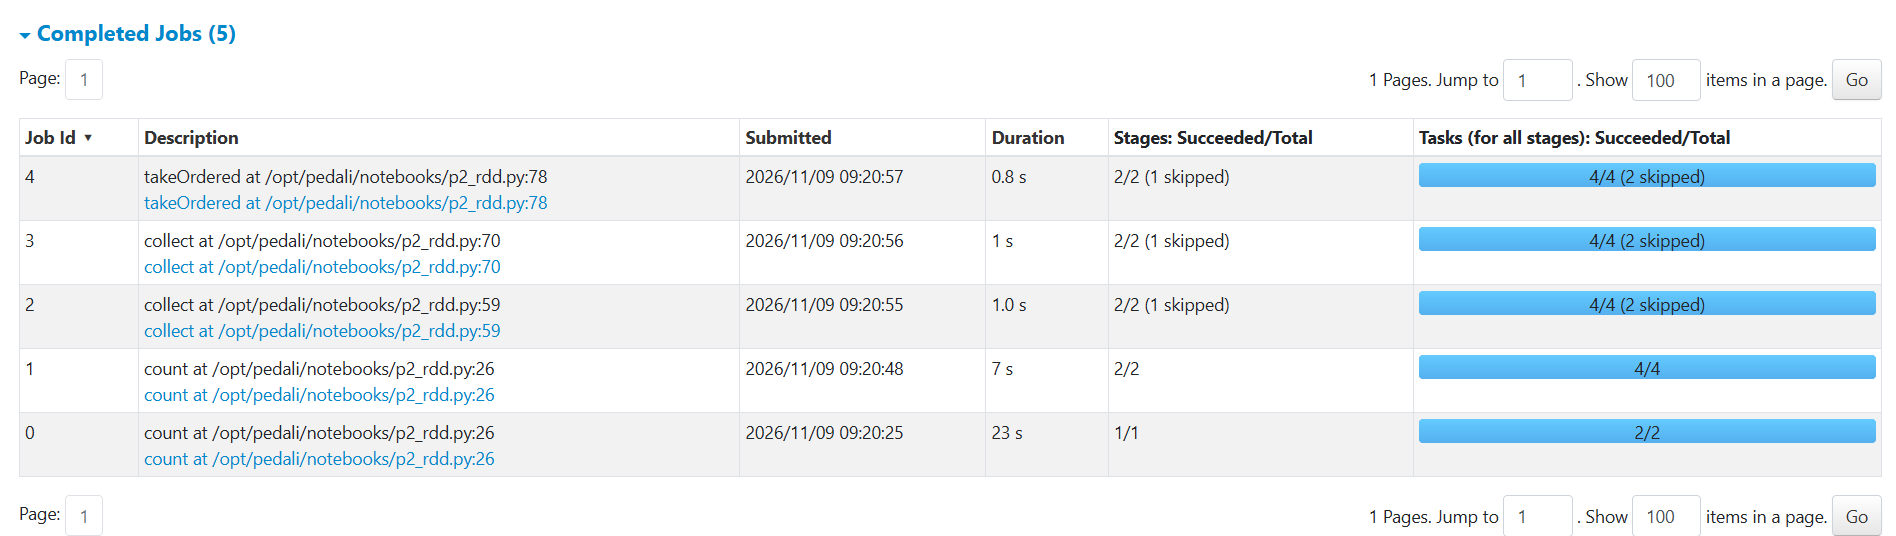
\includegraphics[width=0.8\linewidth]{p2_jobs.png}
  \caption{Les 5 jobs de \code{p2_rdd.py}, un par action.}
\end{subfigure}\\[2mm]
\begin{subfigure}[b]{\linewidth}\centering
  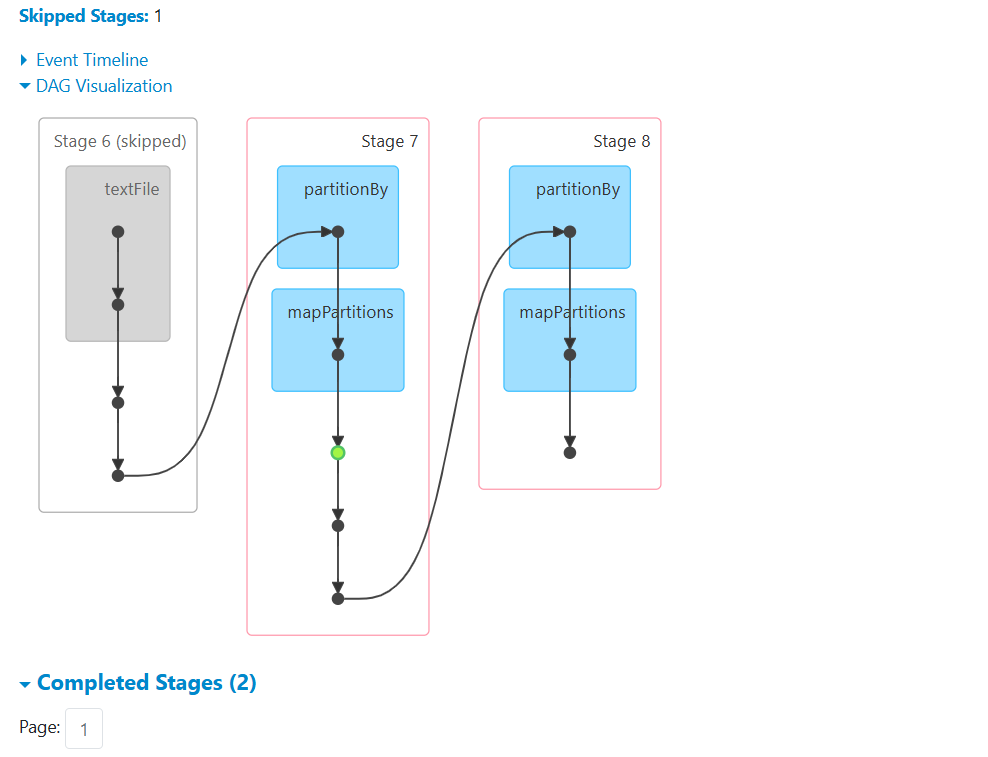
\includegraphics[width=0.36\linewidth]{p2_dag.png}
  \caption{DAG d'une agrégation (job 3, \code{aggregateByKey}) : 3 stages, dont un
  \emph{skipped}.}
\end{subfigure}
\caption{Spark UI de la Partie 2 (port 4040).}
\label{fig:p2-ui}
\end{figure}

\textbf{Nombre de stages.} Le job~0 (\code{count} des lignes brutes) n'a qu'un stage, car il
n'y a pas de shuffle. Il s'exécute en 2 tâches, une par partition. Le job~1 (\code{count}
des trajets terminés) a 2 stages, à cause du \code{reduceByKey} de dédoublonnage. Les jobs~2
à~4 (CA, durée moyenne, top~5) ont chacun 3 stages, soit 2 frontières de shuffle :
\begin{enumerate}
  \item lecture et dédoublonnage côté map ;
  \item obtention de \code{ended}, puis agrégation partielle ;
  \item agrégation finale.
\end{enumerate}
Le premier stage est \emph{skipped}, car \code{ended} est déjà en cache : le stage~2 le lit
directement en mémoire (point vert dans le stage~7 de la figure).

\textbf{Shuffle provoqué par \code{reduceByKey}.} Pour additionner le CA d'une ville, toutes
ses paires \code{(city, price)} doivent finir sur la même tâche. \code{reduceByKey} procède
en deux temps :
\begin{itemize}
  \item côté \emph{map}, il pré-agrège dans chaque partition (\emph{map-side combine}) et
    écrit des fichiers de shuffle répartis par \texttt{hash(clé) mod n} ;
  \item côté \emph{reduce}, chaque tâche du stage suivant récupère par le réseau les blocs qui
    la concernent.
\end{itemize}
Grâce à la pré-agrégation, seules quelques lignes par partition traversent le réseau (une par
ville) au lieu de 14\,370. C'est ce qui le rend bien plus efficace que \code{groupByKey}.
Le shuffle reste l'opération la plus coûteuse (écriture disque, réseau, sérialisation), et
c'est lui qui découpe le job en stages.

\textbf{Tolérance aux pannes par le lineage.} Spark ne réplique pas les données
intermédiaires : il retient comment chaque partition a été calculée. Si un executor tombe
et qu'une partition de \code{ended} est perdue (le cache n'est pas répliqué), le Driver la
recalcule en rejouant uniquement son lineage : relecture du bloc S3 correspondant, puis
\code{flatMap}, \code{filter} et \code{reduceByKey}. Pour une dépendance étroite, seule la
partition perdue est recalculée. Pour une dépendance large, Spark réexécute les tâches
\emph{map} dont les fichiers de shuffle ont disparu. Les autres partitions ne sont pas
touchées.

\textit{Remarque :} avec 2 partitions seulement, le stage de lecture n'occupe que 2 des
4 cœurs. Un \code{sc.textFile(path, minPartitions=4)} utiliserait tout le cluster.

% ============================================================================
\section{Partie 3 -- Spark SQL et DataFrames}

\subsection{Schémas explicites}

\code{notebooks/p3_dataframes.py} lit les deux sources avec un \code{StructType}, sans
inférence. Le schéma \code{TRIP_SCHEMA} (13 champs) sera réutilisé tel quel dans
\code{from_json} en Partie 4. \code{event_time} est lu comme chaîne ISO~8601, puis converti
avec \code{to_timestamp} : un format inattendu donne \code{null} au lieu de faire échouer la
lecture.

\begin{lstlisting}[style=py]
TRIP_SCHEMA = StructType([
    StructField("trip_id", StringType()), StructField("user_id", StringType()),
    StructField("vehicle_id", StringType()), StructField("vehicle_type", StringType()),
    StructField("start_station", StringType()), StructField("end_station", StringType()),
    StructField("city", StringType()), StructField("status", StringType()),
    StructField("duration_s", IntegerType()), StructField("distance_km", DoubleType()),
    StructField("battery_pct", IntegerType()), StructField("price_mad", DoubleType()),
    StructField("event_time", StringType())])
trips = spark.read.schema(TRIP_SCHEMA).json(HISTORY).withColumn("event_ts", F.to_timestamp("event_time"))
stations = spark.read.schema(STATION_SCHEMA).option("multiLine", True).json(STATIONS)   # 8 champs
\end{lstlisting}

Le schéma explicite présente trois avantages :
\begin{itemize}
  \item il évite une passe complète de lecture pour inférer les types ;
  \item il fixe des types stables, par exemple \code{duration_s} en entier même quand les
    premières lignes valent \code{null} ;
  \item c'est indispensable en streaming, où l'inférence est impossible.
\end{itemize}
\code{stations.json} est lu avec \code{multiLine} : 400 stations, aucune orpheline après
jointure.

\subsection{Chiffre d'affaires : API DataFrame et SQL}

\begin{lstlisting}[style=py]
revenue_df = ended.groupBy("city").agg(F.round(F.sum("price_mad"), 2).alias("ca_mad"))
ended.createOrReplaceTempView("trips_ended")
revenue_sql = spark.sql("SELECT city, ROUND(SUM(price_mad), 2) AS ca_mad FROM trips_ended GROUP BY city ORDER BY city")
\end{lstlisting}
Les deux versions donnent exactement les valeurs du tableau~\ref{tab:ca}. La durée moyenne
et le top~5 recalculés en DataFrame sont aussi identiques à la Partie~2. SQL et DataFrame
passent par le même optimiseur Catalyst et produisent le même plan d'agrégation (la version
SQL ajoute seulement un tri) : ce sont deux façons d'écrire la même requête.

\subsection{Jointure avec le référentiel stations}

Les trajets terminés sont joints aux stations sur la station de départ (jointure
\code{left}), puis agrégés par ville et type de zone.

\begin{table}[!htbp]
\centering\small
\begin{tabular}{@{}lrrrr@{}}
\toprule
\textbf{Type de zone} & \textbf{Casablanca} & \textbf{Marrakech} & \textbf{Rabat} & \textbf{Tanger} \\
\midrule
résidentiel        & 3\,077 \; (91,5) & 1\,069 \; (31,6) & 706 \; (20,3) & 1\,009 \; (29,8) \\
centre d'affaires  & 1\,021 \; (30,9) &    683 \; (20,7) & 465 \; (14,3) &    428 \; (12,9) \\
plage              &    804 \; (24,0) &    165 \; (5,1)  & 394 \; (11,9) &    103 \; (3,6) \\
gare               &    540 \; (16,0) &    297 \; (9,1)  & 503 \; (15,1) &    288 \; (8,8) \\
tourisme           &    506 \; (15,4) &    353 \; (10,5) & 545 \; (16,0) &    173 \; (5,3) \\
université         &    499 \; (14,7) &    246 \; (7,0)  & 305 \; (9,1)  &    191 \; (5,9) \\
\bottomrule
\end{tabular}
\caption{Nombre de trajets terminés et, entre parenthèses, CA en milliers de MAD, par type
de zone de la station de départ.}
\label{tab:zone}
\end{table}

Les zones résidentielles dominent partout, ce qui reflète leur part dans le référentiel
(39\,\% des stations). À Rabat, les zones touristiques et les gares arrivent juste derrière.
Aucun trajet n'est orphelin (0 station de départ inconnue).

\subsection{UDF \texttt{trip\_band} contre \texttt{when/otherwise}}

\begin{lstlisting}[style=py]
def trip_band_py(d):                       # UDF Python : exécutée ligne par ligne hors de la JVM
    if d is None: return None
    return "court" if d < 600 else ("moyen" if d <= 1800 else "long")
trip_band_udf = F.udf(trip_band_py, StringType())
trip_band_col = (F.when(F.col("duration_s").isNull(), F.lit(None))     # expression native Catalyst
                  .when(F.col("duration_s") < 600, "court")
                  .when(F.col("duration_s") <= 1800, "moyen").otherwise("long"))
\end{lstlisting}

Les deux versions donnent la même répartition, vérifiée par un \code{assert} : court
2\,580 (18,0\,\%), moyen 9\,784 (68,1\,\%), long 2\,006 (14,0\,\%). La version native est
pourtant \textbf{8,4 fois plus rapide} (1,53~s contre 12,90~s, 4,1 fois avec 4 partitions de
shuffle, voir tableau~\ref{tab:temps}). Plusieurs raisons l'expliquent :
\begin{itemize}
  \item \textbf{Sérialisation.} Avec l'UDF, chaque ligne quitte la JVM : elle est sérialisée
    (pickle) vers un processus Python, évaluée, puis renvoyée.
  \item \textbf{Boîte noire pour Catalyst.} L'UDF apparaît dans le plan comme un nœud
    \code{BatchEvalPython}. Catalyst ne peut ni l'optimiser ni la simplifier, et elle coupe
    le \emph{whole-stage code generation}.
  \item \textbf{Expression native.} \code{when/otherwise} devient un \code{CaseWhen}. Il est
    compilé en bytecode Java avec le reste du stage et s'applique directement au format
    binaire Tungsten, sans copie ni changement de processus.
\end{itemize}
Si une UDF est inévitable, une \code{pandas_udf} (vectorisée par Apache Arrow) limite ce coût.

\subsection{Couche Silver en Parquet partitionné par ville}

La couche Silver conserve tous les statuts, dédoublonnés sur \code{(trip_id, status)} :
c'est elle que la Partie~6 relira. On y ajoute la colonne \code{trip_band}, et l'écriture
se fait avec \code{partitionBy("city")} dans \path{s3a://lake/silver/trips_history/}.
Résultat : \textbf{50\,000 lignes} (les 1\,000 doublons sont éliminés) réparties en
16 fichiers Snappy (4 villes $\times$ 4 tâches). Le tout pèse 1,9~Mo, contre 15,9~Mo
pour le JSON brut, soit \textbf{8,4 fois moins} grâce au format colonne et à la
compression. Le partitionnement permet le \emph{partition pruning} : une requête filtrée
sur \code{city = 'Rabat'} ne lit que le dossier \code{city=Rabat/}.

\begin{figure}[!htbp]
\centering
\begin{subfigure}[b]{0.49\linewidth}
  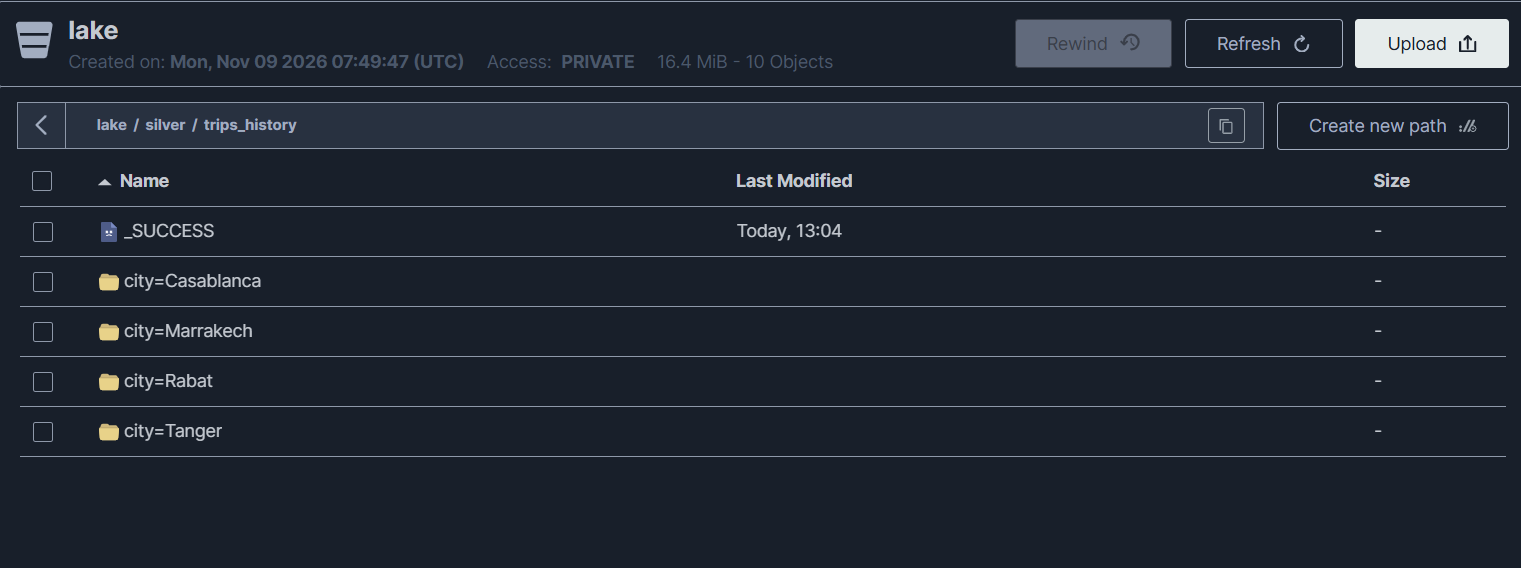
\includegraphics[width=\linewidth]{p3_minio_silver.png}
  \caption{Un dossier par ville.}
\end{subfigure}\hfill
\begin{subfigure}[b]{0.49\linewidth}
  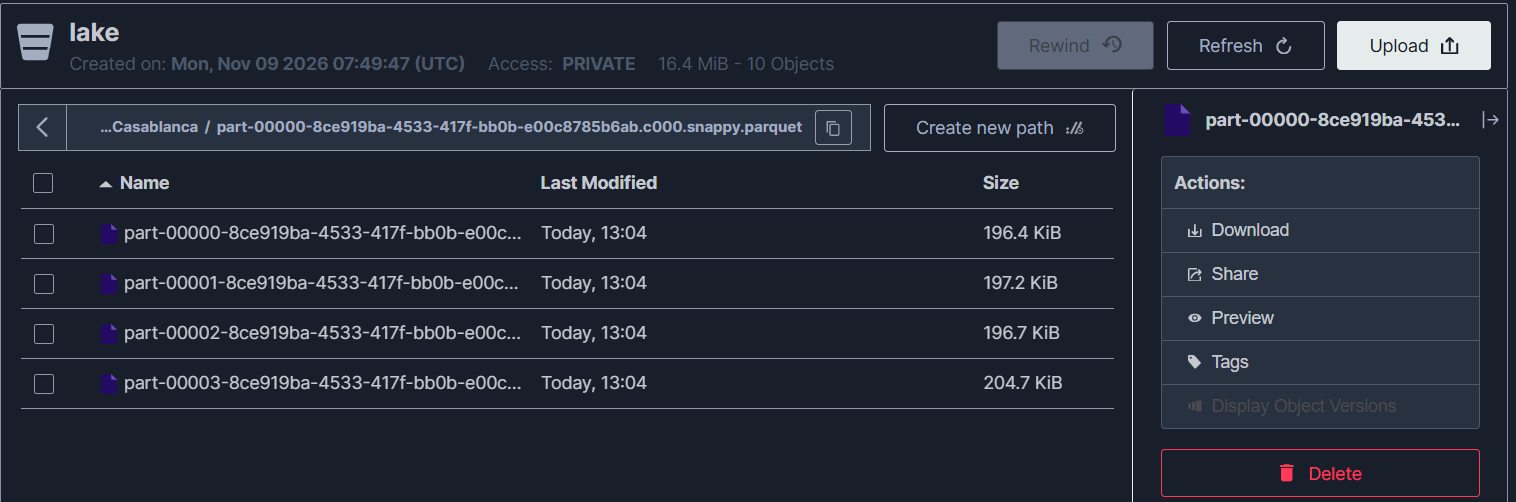
\includegraphics[width=\linewidth]{p3_minio_parquet.png}
  \caption{Fichiers Parquet de \code{city=Casablanca}.}
\end{subfigure}
\caption{Couche Silver dans la console MinIO.}
\label{fig:p3-minio}
\end{figure}

\begin{lstlisting}[style=out,title={\footnotesize \texttt{mc ls --recursive local/lake/} (extrait)}]
[2026-11-22 07:33:39 UTC]  15MiB STANDARD bronze/history/trips_history.jsonl
[2026-11-22 07:33:47 UTC]  84KiB STANDARD bronze/ref/stations.json
[2026-11-22 07:38:48 UTC]     0B STANDARD silver/trips_history/_SUCCESS
[2026-11-22 07:38:45 UTC] 197KiB STANDARD silver/trips_history/city=Casablanca/part-00000-45695d36-....snappy.parquet
...                                       (4 fichiers par ville, 16 au total)
[2026-11-22 07:38:48 UTC]  74KiB STANDARD silver/trips_history/city=Tanger/part-00003-45695d36-....snappy.parquet
\end{lstlisting}

\subsection{Plan d'exécution : \texttt{explain(True)} sur la jointure}

Sortie complète de \code{plan_df.explain(True)} (jointure des trajets \code{ENDED} avec les
stations, puis comptage par ville et type de zone) :

\lstinputlisting[style=out,basicstyle=\ttfamily\scriptsize]{sorties/p3_explain.txt}

\begin{itemize}
  \item \textbf{Plan logique} (\emph{Parsed}, puis \emph{Analyzed}). Le plan \emph{parsed}
    reprend littéralement notre code : \code{Filter} sur les trajets, \code{Join LeftOuter},
    \code{Aggregate}. Les colonnes n'y sont pas encore résolues (\code{'city}). L'analyseur
    les rattache ensuite aux schémas et vérifie les types (\code{nb_trajets: bigint}).
  \item \textbf{Plan optimisé par Catalyst.} Trois optimisations apparaissent :
    \begin{itemize}
      \item \emph{column pruning} : il ne garde que \code{start_station}, \code{city} et
        \code{status} sur 13 colonnes, et le calcul inutile de \code{event_ts}
        (\code{to_timestamp}) disparaît ;
      \item \emph{predicate pushdown} : le filtre \code{status = ENDED} descend jusqu'au scan
        (\code{PushedFilters}) ;
      \item \emph{inférence de filtres} : il ajoute \code{isnotnull(station_id)}, puisqu'une
        clé nulle ne peut pas joindre.
    \end{itemize}
  \item \textbf{Stratégie physique : \code{BroadcastHashJoin} (BuildRight).} La table des
    stations (84~Ko) est sous le seuil \code{spark.sql.autoBroadcastJoinThreshold} (10~Mo).
    Spark l'envoie donc entière à chaque executor (\code{BroadcastExchange}), et les trajets
    sont joints sur place, sans shuffle. Avec deux grosses tables, on aurait eu un
    \code{SortMergeJoin} avec deux \code{Exchange} et deux tris. Le seul shuffle du plan est
    celui de l'agrégation, faite en deux phases : \code{partial_count} avant l'\code{Exchange}
    et \code{count} après. \code{AdaptiveSparkPlan} indique qu'AQE peut encore réviser le
    plan à l'exécution, par exemple pour fusionner les 200 partitions.
\end{itemize}

\begin{figure}[!htbp]
\centering
\begin{subfigure}[b]{0.5\linewidth}\centering
  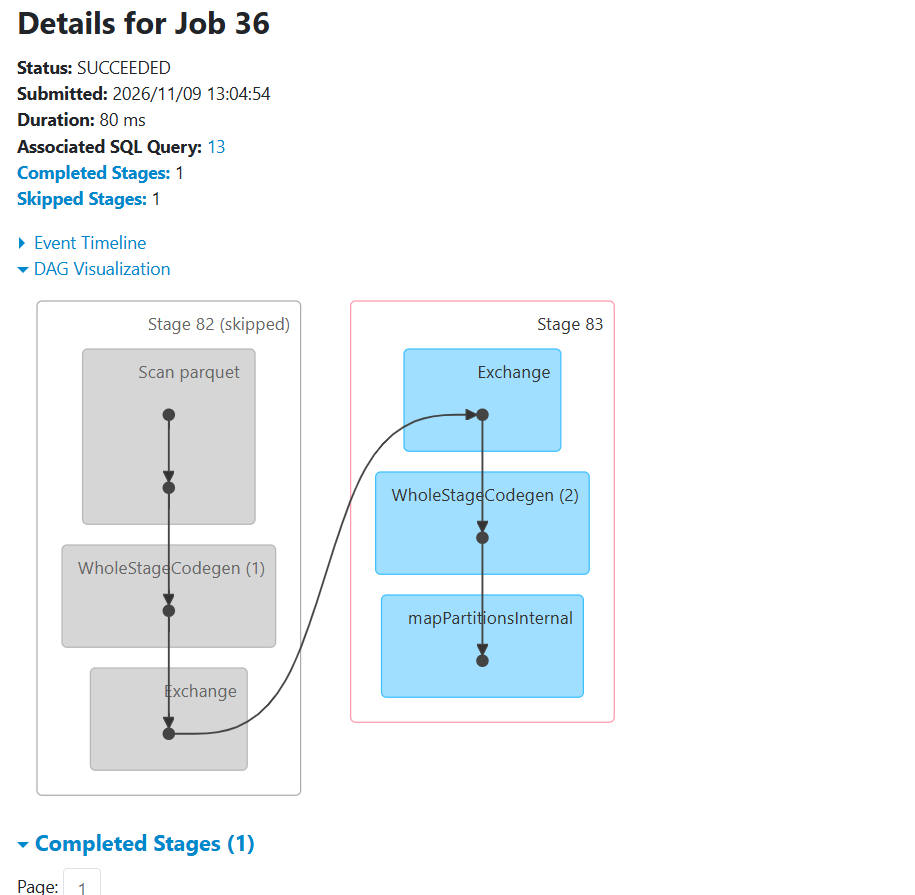
\includegraphics[height=7.4cm]{p3_dag.png}
  \caption{DAG du job~36 : relecture de la couche Silver.}
\end{subfigure}\hfill
\begin{subfigure}[b]{0.38\linewidth}\centering
  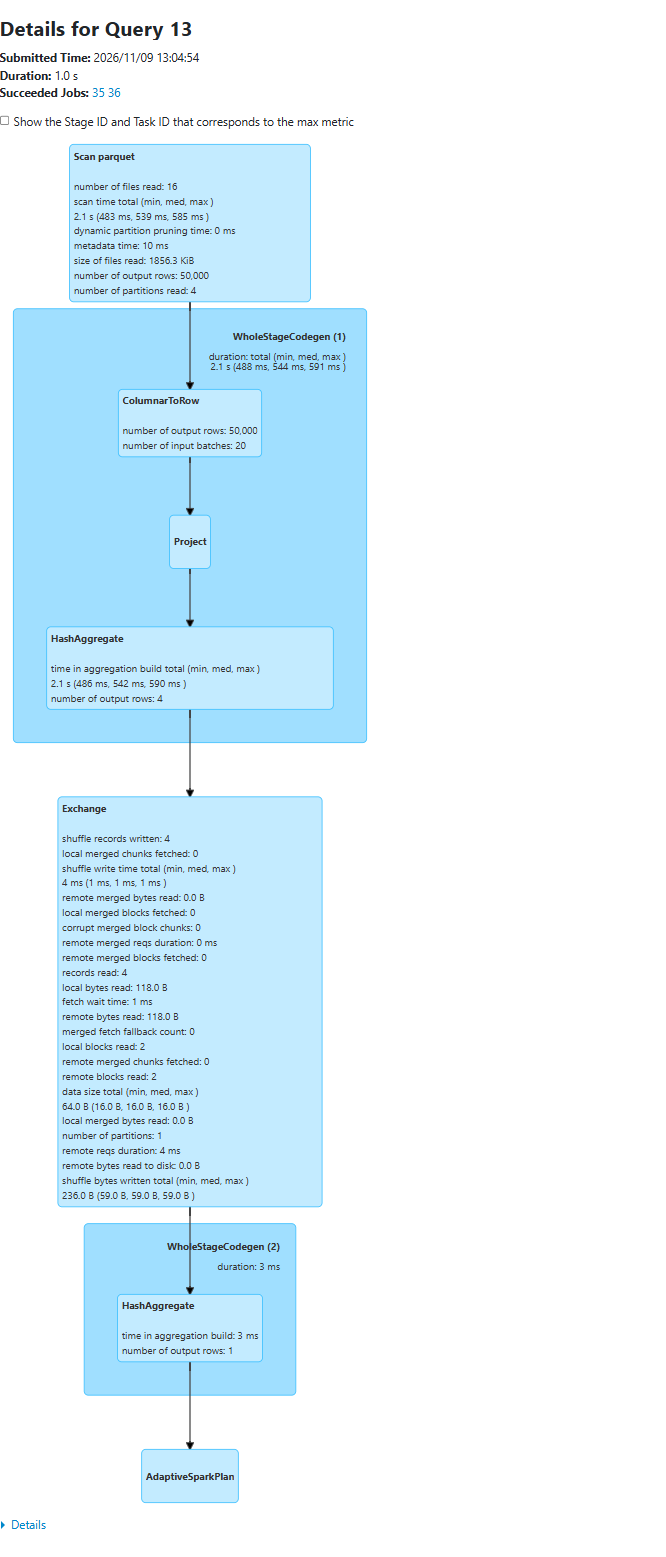
\includegraphics[height=7.4cm]{p3_sql.png}
  \caption{Onglet SQL, requête~13.}
\end{subfigure}
\caption{Spark UI de la Partie 3 : comptage de la couche Silver relue en Parquet. Le scan lit
16 fichiers (1\,856~Kio, 50\,000 lignes, 4 partitions de ville) en lots colonnes
(\code{ColumnarToRow}). Le comptage se fait en deux phases, \code{HashAggregate} partiel puis
final, autour d'un \code{Exchange}.}
\label{fig:p3-ui}
\end{figure}

\begin{figure}[!htbp]
\centering
\begin{subfigure}[b]{\linewidth}\centering
  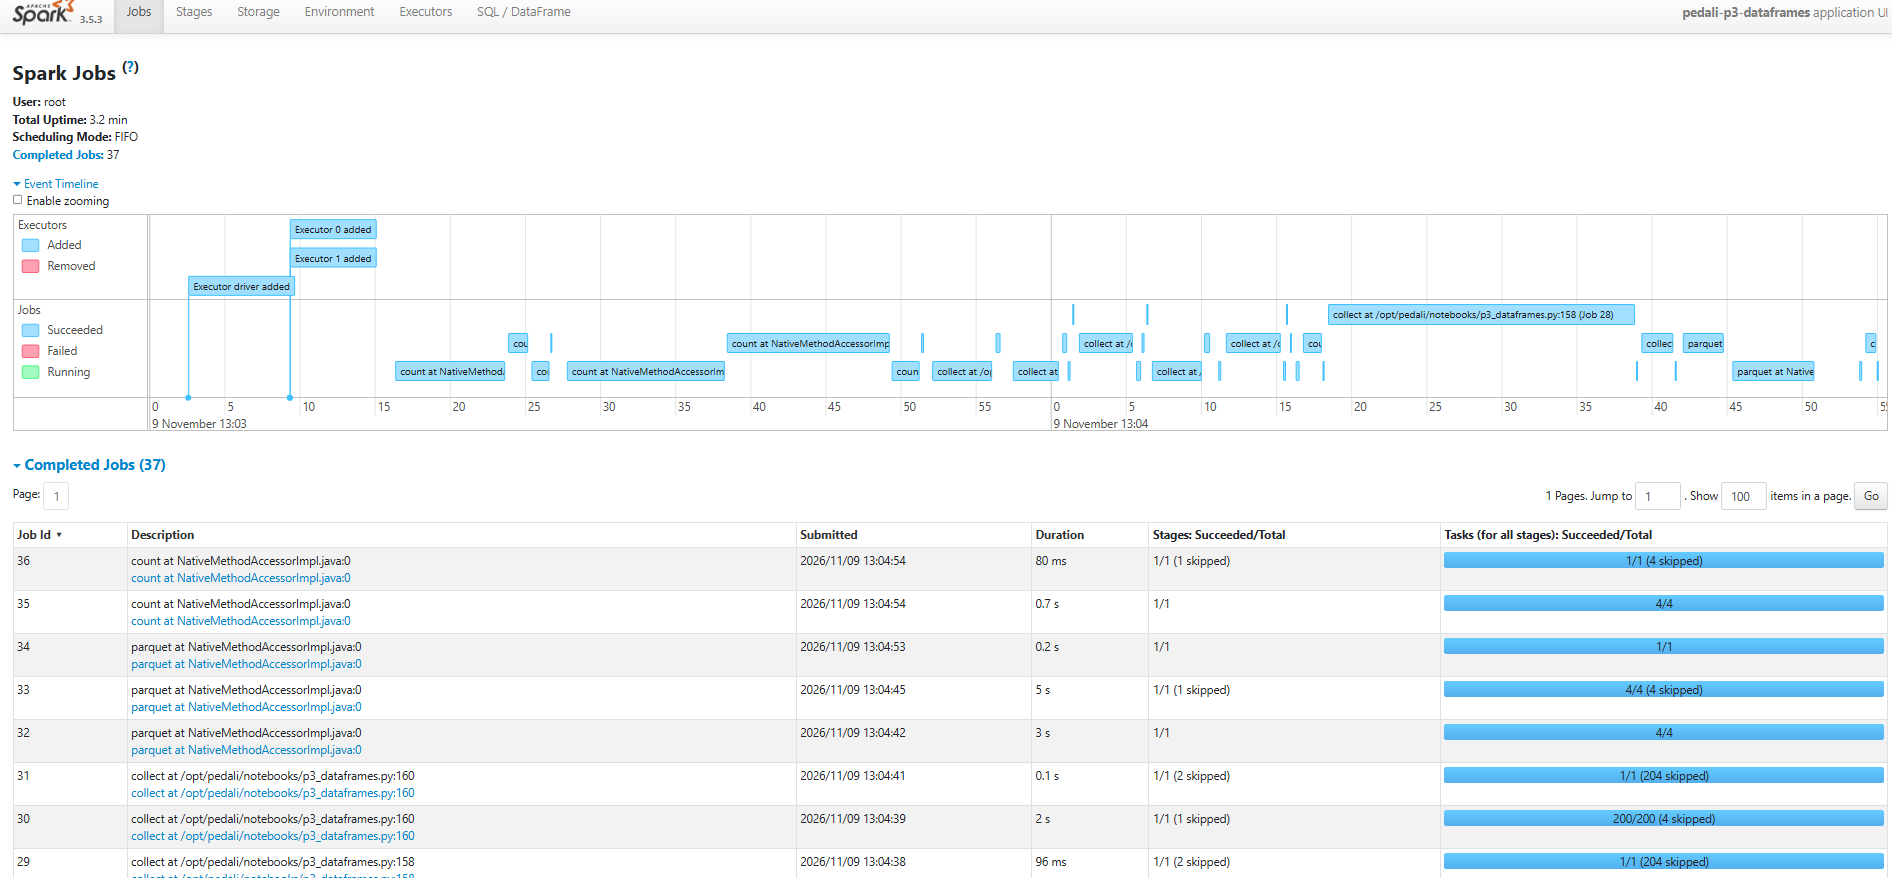
\includegraphics[width=0.8\linewidth]{p3_jobs1.png}
  \caption{Chronologie et jobs 29 à 36.}
\end{subfigure}\\[1mm]
\begin{subfigure}[b]{0.49\linewidth}
  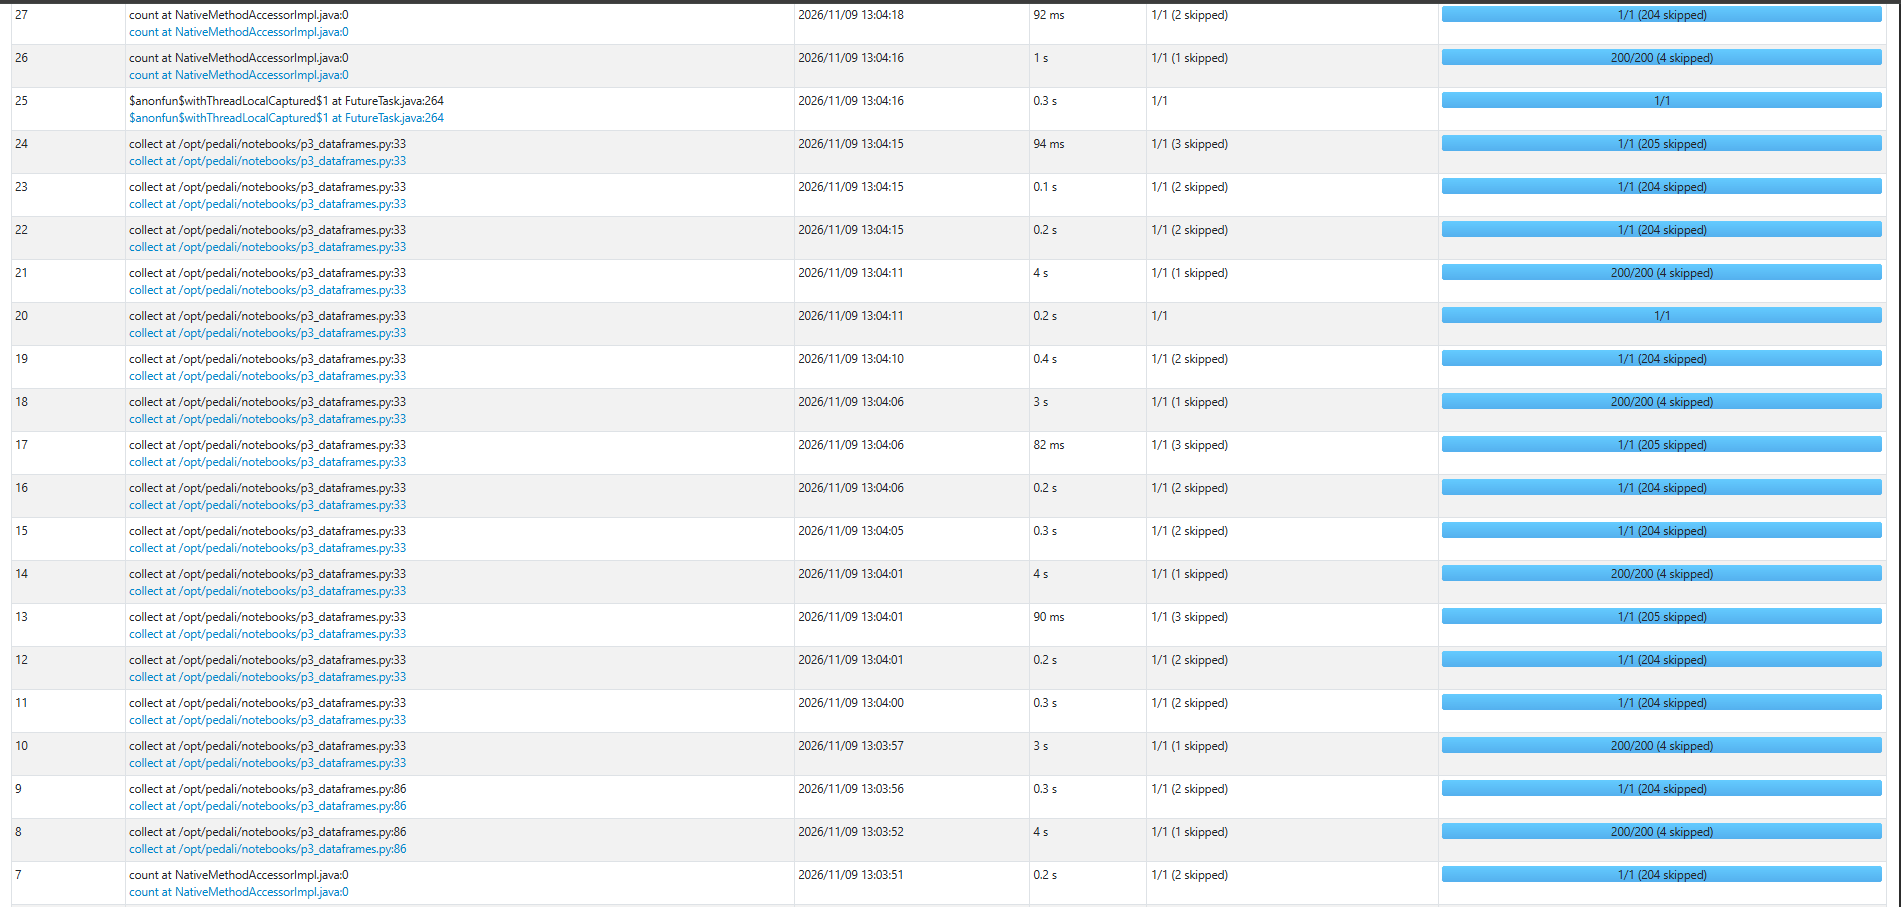
\includegraphics[width=\linewidth]{p3_jobs2.png}
  \caption{Jobs 7 à 27.}
\end{subfigure}\hfill
\begin{subfigure}[b]{0.49\linewidth}
  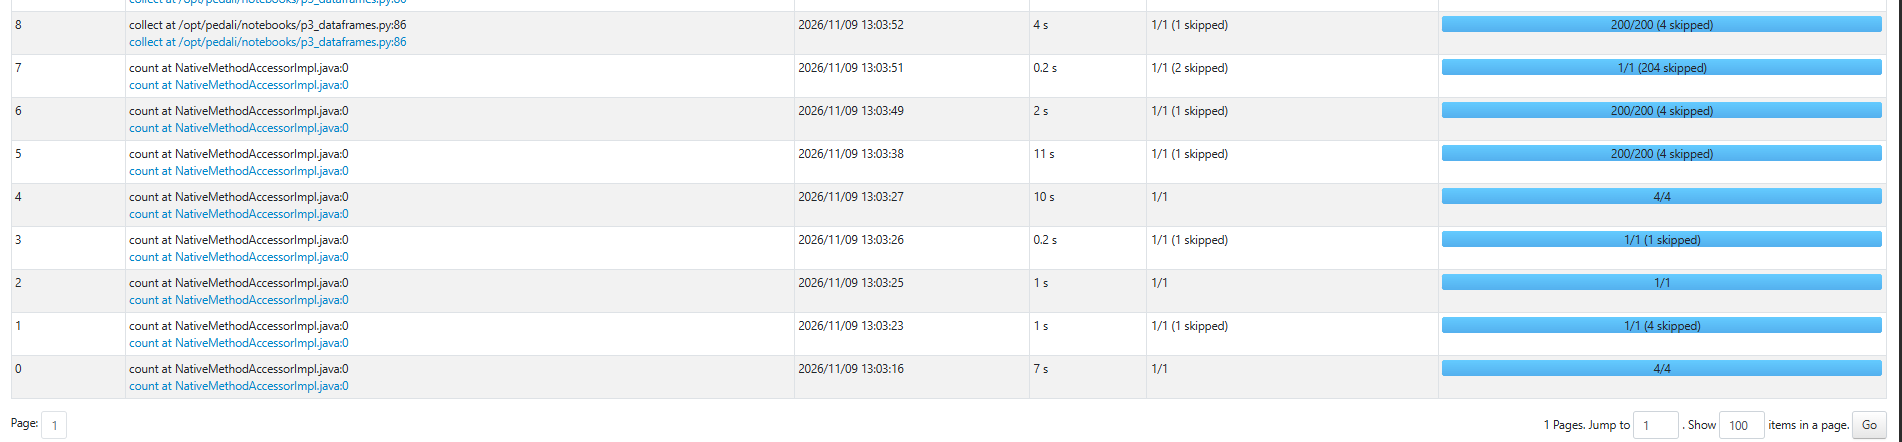
\includegraphics[width=\linewidth]{p3_jobs3.png}
  \caption{Jobs 0 à 8.}
\end{subfigure}
\caption{Les 37 jobs de \code{p3_dataframes.py} dans la Spark UI. Les stages à
\textbf{200/200 tâches} correspondent à \code{spark.sql.shuffle.partitions = 200}, la valeur
par défaut.}
\label{fig:p3-jobs}
\end{figure}

\subsection{RDD, DataFrame et Dataset}

\begin{table}[!htbp]
\centering\small
\begin{tabularx}{\linewidth}{@{}l X X X@{}}
\toprule
 & \textbf{RDD} & \textbf{DataFrame} & \textbf{Dataset} \\
\midrule
Typage & Objets sans schéma (dict Python) & Schéma connu, vérifié à l'exécution & Typé à la compilation (Scala/Java) \\
Optimiseur & Aucun : on exécute ce qu'on écrit & Catalyst : pruning, pushdown, choix de jointure & Catalyst, mais lambdas opaques \\
Exécution & Lambdas Python, données sérialisées vers Python & Tungsten : format binaire, codegen, tout en JVM & Tungsten via \emph{Encoders} \\
PySpark & Oui & Oui (= \code{Dataset[Row]}) & Non (Python est dynamique) \\
\bottomrule
\end{tabularx}
\caption{Comparaison des trois API.}
\end{table}

\begin{table}[!h]
\centering\small
\begin{tabular}{@{}lrrr@{}}
\toprule
\textbf{Opération (secondes)} & \textbf{RDD (P2)} & \textbf{DataFrame, 200 part.} & \textbf{DataFrame, 4 part.} \\
\midrule
Lecture + \code{count} (démarrage inclus) & 10,34 & 8,77 & 9,02 \\
Filtre \code{ENDED} + dédoublonnage + cache & 7,38 & 12,97 & 5,41 \\
CA par ville (SQL) & 0,74 & 3,54 (3,22) & 1,33 (1,24) \\
Durée moyenne ville $\times$ véhicule & 0,66 & 2,95 & 1,34 \\
Top 5 des stations & 0,68 & 2,98 & 1,03 \\
\code{trip_band} : UDF / \code{when} & -- & 12,90 / 1,53 & 2,51 / 0,61 \\
\bottomrule
\end{tabular}
\caption{Temps mesurés le 22/11/2026, même cluster, une exécution chacun. La dernière
colonne relance le même script avec \code{spark.sql.shuffle.partitions=4}
(\code{report/sorties/p3_dataframes_shuffle4.txt}).}
\label{tab:temps}
\end{table}

\textbf{Lecture des mesures.} Les trois API donnent des résultats identiques, mais les temps
ne suivent pas l'intuition « DataFrame plus rapide » : sur nos 16~Mo, les RDD agrègent plus
vite. L'explication tient aux coûts fixes, visibles dans la Spark UI :
\begin{itemize}
  \item le DataFrame \code{ended} est mis en cache juste après un \code{dropDuplicates}, donc
    avec les 200 partitions du shuffle ;
  \item chaque agrégation lance alors 200 tâches pour 14\,370 lignes, soit environ
    70 lignes par tâche (figure~\ref{fig:p3-jobs}) ;
  \item chaque action paie en plus l'analyse, l'optimisation et la génération de code de
    Catalyst, quelques centaines de millisecondes non amorties sur si peu de données.
\end{itemize}
Avec 4 partitions, les agrégations passent sous 1,4~s, et le dédoublonnage devient plus
rapide qu'en RDD (5,41~s contre 7,38~s), car il ne repasse pas par Python.

L'avantage structurel du DataFrame est visible dans deux cas :
\begin{itemize}
  \item l'UDF contre l'expression native (4 à 8 fois plus rapide) ;
  \item la lecture : le plan ne lit que 3 colonnes sur 13 et filtre dès le scan, alors que
    le RDD parse en Python chaque ligne JSON complète.
\end{itemize}
Ces gains croissent avec le volume : à plusieurs gigaoctets, les coûts fixes deviennent
négligeables, contrairement à la sérialisation Python des RDD. Le Dataset offrirait en plus
la sûreté de typage en Scala, mais ses lambdas typées (\code{map}, \code{filter}) restent
opaques pour Catalyst. Nous retenons donc les DataFrames pour la suite du projet : streaming
en Partie~4 et GraphFrames en Partie~6. Il faudra régler \code{spark.sql.shuffle.partitions}
au volume réel.

% ============================================================================
\section*{Bilan du jalon 1}
\addcontentsline{toc}{section}{Bilan du jalon 1}

Le cluster Spark (1 Master, 2 Workers), Kafka (topic \code{trips}, 3 partitions) et MinIO
(bucket \code{lake}) sont déployés et reproductibles avec Docker Compose. L'historique est
analysé de bout en bout, en RDD puis en DataFrame/SQL, avec des résultats concordants. La
couche Silver est écrite en Parquet partitionné par ville. Prochaines étapes (jalon 2,
20/12/2026) :
\begin{itemize}
  \item brancher \code{producer.py} sur Kafka et passer en Structured Streaming ;
  \item produire les couches \code{silver/trips_clean} et \code{gold} en Delta Lake ;
  \item construire le graphe stations--trajets avec GraphFrames et GraphX.
\end{itemize}
Les sorties console complètes des Parties 2 et 3 (dont \code{explain(True)} et
\code{mc ls --recursive local/lake/}) sont versionnées dans \code{report/sorties/}.

\end{document}
